\part{Introduction}
\section{property of the KPO model Hamiltonian}
次のKPO Hamiltonianを考える:
\begin{align}
    \hat{H}_{\rm{KPO}}&=\hat{H}_0 +p\hat{V}\\[5pt]
    \hat{H}_0&=\Delta \hat{a}^\dagger\hat{a} + \frac{\chi}{2} \hat{a}^\dagger\hat{a}^\dagger\hat{a}\hat{a}\\[5pt]
    \hat{V}&=(\hat{a}^2 + \hat{a}^{\dagger 2})
\end{align}
ここで,$\hat{H}_0$は対角化できており,エネルギー固有状態とエネルギー固有値は以下で与えられる:
\begin{align}
    \hat{H}_0&=\Delta \hat{n} + \frac{\chi}{2}\hat{n}(\hat{n}-1) \\[5pt]
    \hat{H}_0\ket{n}&=E_n\ket{n},\ \ \ 
    E_n = \Delta n + \frac{\chi}{2}n(n-1)
\end{align}
このとき,基底状態と各励起状態が縮退する条件は固有エネルギーが0となるとき,すなわち,
\begin{align}
        E_n &= \Delta n + \frac{\chi}{2}n(n-1) =0\\[10pt]
        \Delta &= -\frac{\chi}{2}(n-1)
\end{align}
となる.


\section{いくつかの数値計算結果}
上に示したKPOのHamiltonianの興味深い性質を確認するために,次のGKSL型マスター方程式を用いて数値計算を行った:
\begin{align}\label{Eq.GKSL}
\frac{\partial\rho}{\partial t} = -i\left[\hat{H}_{\rm{KPO}} 
,\ \rho\right] 
+\frac{\gamma}{2} \left (2\hat a \rho \hat a^\dagger - \left\{ \hat a^\dagger \hat a, \rho \right\}\right).
\end{align}
図\ref{fig:kpo_steady_0.14}, \ref{fig:kpo_steady_0.0001}はマスター方程式の定常状態$\hat{\rho}_{\rm{ss}}\equiv\frac{\partial\rho}{\partial t}=0$を数値計算によって求め,その平均光子数$\braket{\hat{a}^\dagger\hat{a}}\equiv\tr[\hat{\rho}_{\rm{ss}}\hat{a}^\dagger\hat{a}]$をパラメトリックドライブ$p$,detuning $\Delta$をそれぞれ変え,求めた.図に示すように,DetuningがKerr係数$\chi$とが
\begin{equation}\label{on-resonant}
    \Delta = -\frac{\chi}{2}(n-1)
\end{equation}
の条件(これを共鳴条件と呼ぶ.)を満たすとき,わずかなパラメトリックドライブでさえ,平均光子数が急激に増加していることがわかる.


\begin{figure}[h]
\centering
		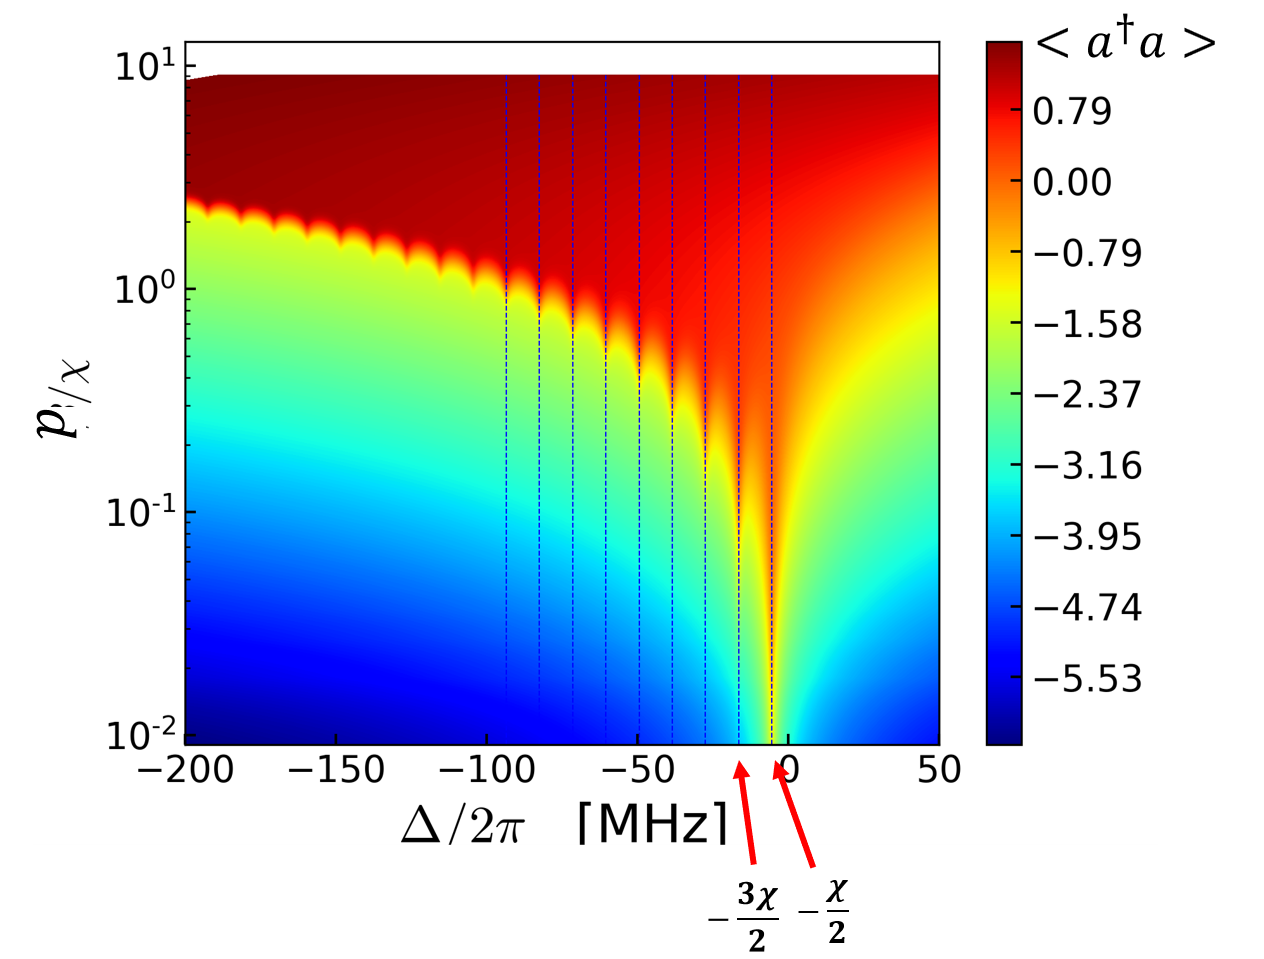
\includegraphics[width=10cm]{file/fig/numerical_steady/spect_number_td2D_Keer_11_decay_1.4.png} \\
\caption{$z$軸は平均光子数に常用対数を取ったもの.$Kerr / 2\pi = 11$ MHz, $\gamma / 2\pi = 1.4$ MHz. $x$軸はdetuning, $y$軸はパラメトリックドライブを表す.}
\label{fig:kpo_steady_0.14}
\end{figure}


\begin{figure}[h]
\centering
		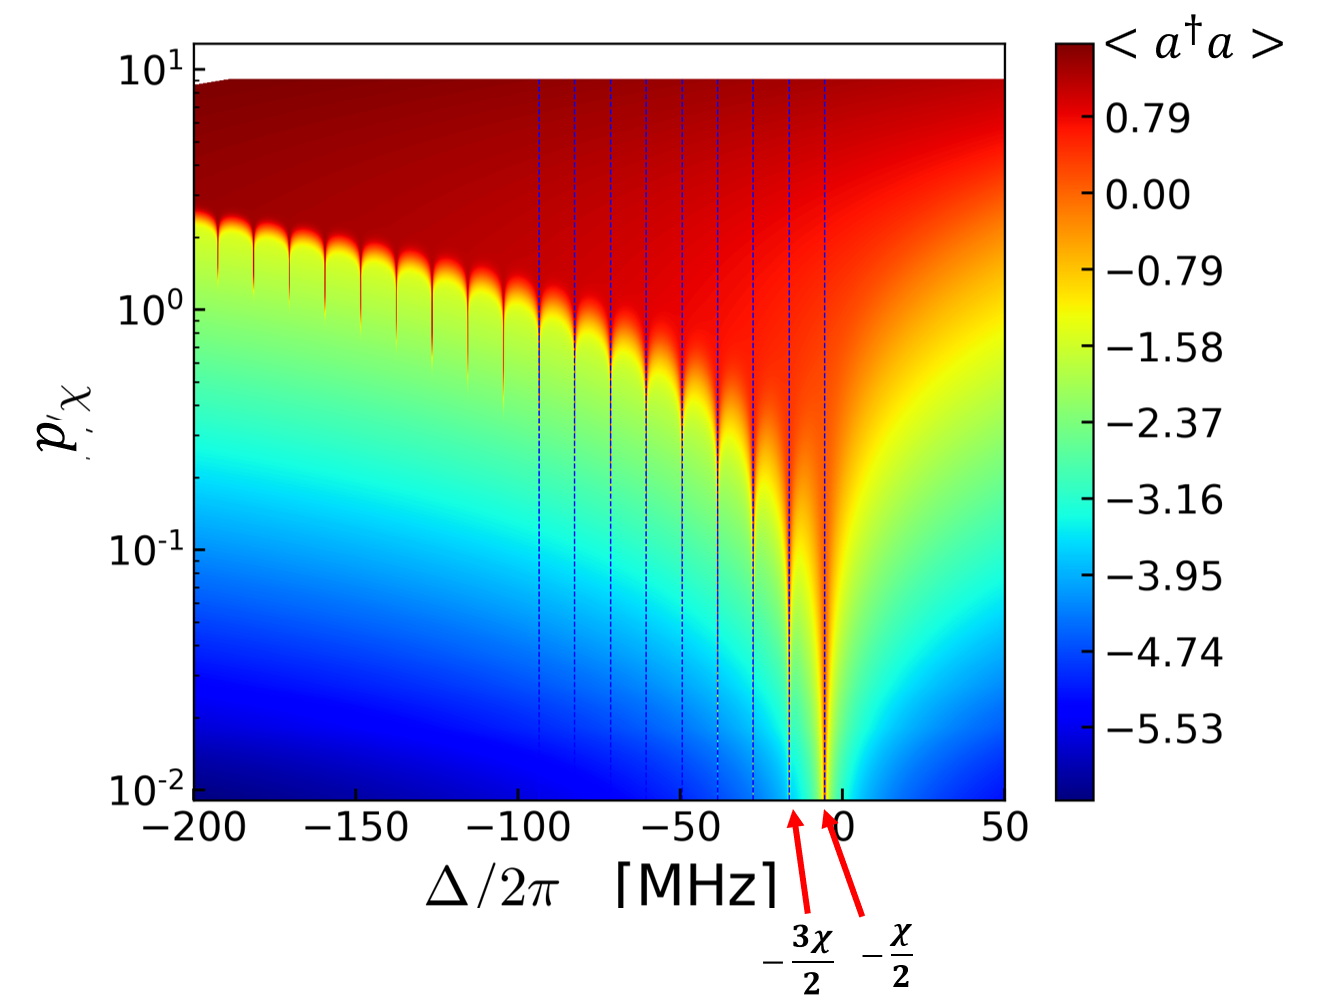
\includegraphics[width=10cm]{file/fig/numerical_steady/spect_number_td2D_Keer_11_decay_0.0001.png} \\
\caption{$z$軸は平均光子数に常用対数を取ったもの.$Kerr / 2\pi = 11$ MHz, $\gamma / 2\pi = 0.0001$ MHz. $x$軸はdetuning, $y$軸はパラメトリックドライブを表す.}
\label{fig:kpo_steady_0.0001}
\end{figure}


\section{このノートの目的}
このノートでは,なぜ,共鳴条件 Eq.\eqref{on-resonant}を満たすとき,わずかなパラメトリックドライブで,平均光子数が急激に増加しているのかを理論的に解明するためのノートである.理論解析の手法として,時間に依存しない縮退のある場合の摂動論を用いる.また,おまけとして,Schrieffer-Wolff変換やPeter Knight perturbation (断熱消去?)などの摂動論による解析も(あまりうまくはいかなかったが)試みたので,紹介する.

\section{KPO Hamiltonianの行列表示}
KPO Hamiltonianに対して,Detuning $\Delta$を共鳴条件 Eq.\eqref{on-resonant}を満たすようにとる.このとき,摂動Hamiltonian $\hat{V}=(\hat{a}^2 + \hat{a}^{\dagger 2})$は2光子駆動を表しているため,Hamiltonianは偶数サイトと奇数サイトにブロック対角化可能である.今回注目するのは,基底状態と偶数番目の励起状態が縮退する場合であり,図\ref{fig:kpo_effective_model}のような有効模型を考えることができる.
つまり,KPO Hamiltonianを偶数番目のFock状態で展開し,次のように行列で表現することが可能である:
\begin{align}
     \hat{H}_{\rm{KPO}}=
   \bordermatrix{     
    & \bra{0} &  \bra{2} &  \bra{4}&  \bra{6}&  \bra{8}& \cdots& \cdots \cr
   \ket{0}&E_0&\sqrt{2\cdot1}p&0&0&0&\cdots& \cdots\cr
  \ket{2}&\sqrt{2\cdot1}p&E_2&\sqrt{4\cdot3}p&0&0& \cdots& \cdots\cr
  \ket{4}&0&\sqrt{4\cdot3}p&E_4&\sqrt{6\cdot5}p&0& \cdots& \cdots\cr
  \ket{6}&0&0&\sqrt{6\cdot5}p&E_6&\sqrt{8\cdot7}p& \cdots& \cdots\cr
  \ket{8}&0&0&0&\sqrt{8\cdot7}p&E_8& \cdots& \cdots\cr
  \vdots&\vdots & \vdots &\vdots  & \vdots & \dots& \ddots & \vdots \cr
  \vdots&\dots & \dots&\dots &\dots & \dots& \dots  & \vdots\cr
            }
\end{align}


\begin{figure}[h]
\centering
		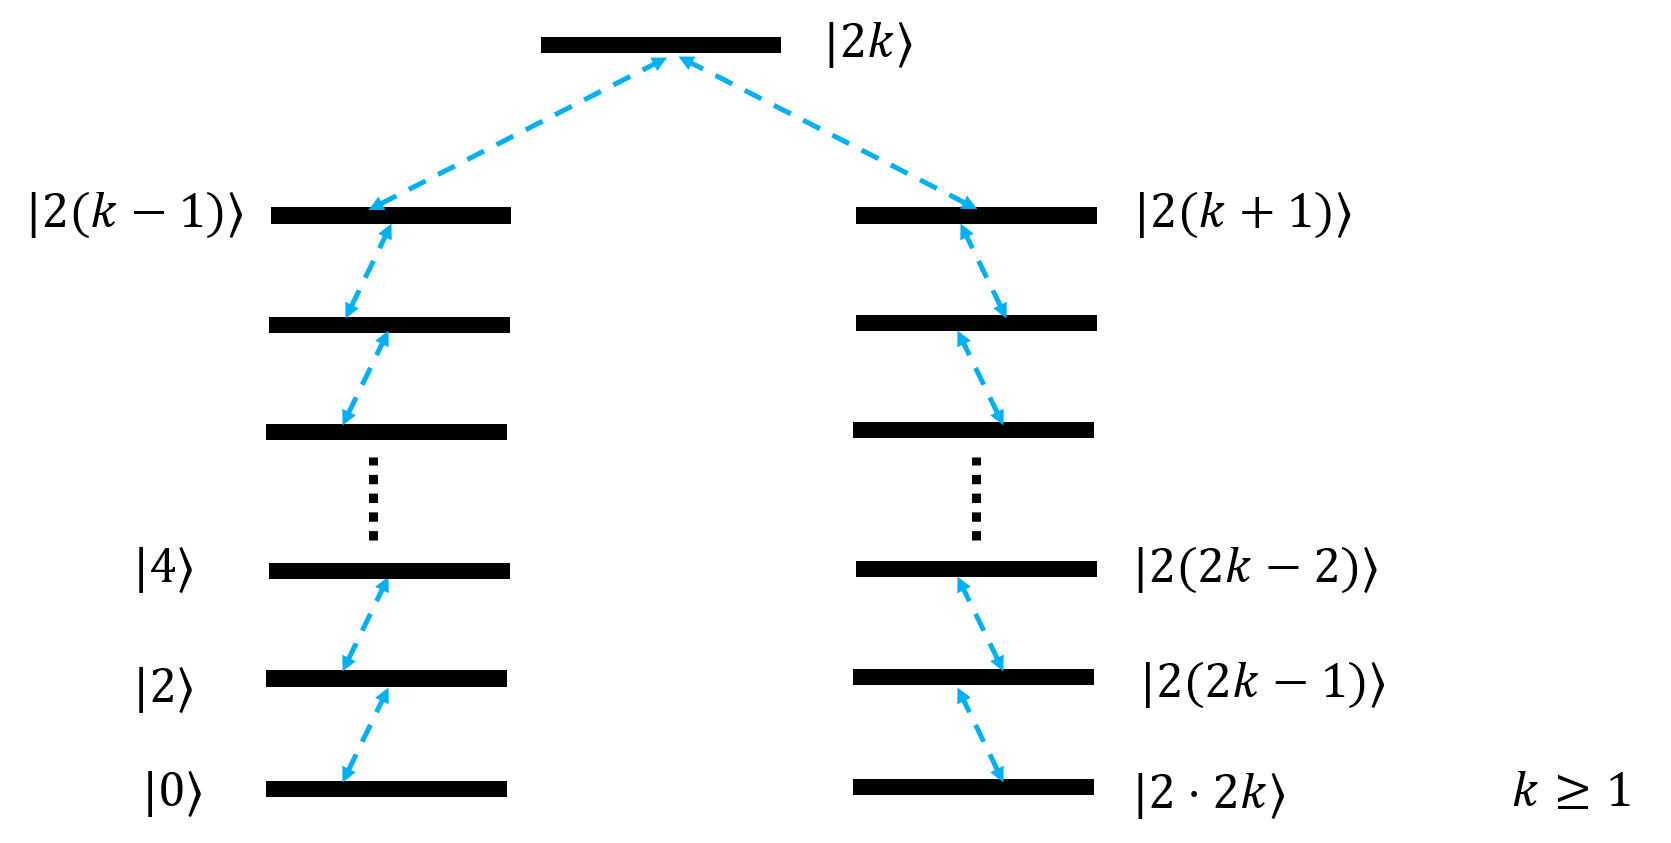
\includegraphics[width=10cm]{file/fig/effective_model/kpo_effective_model.png}\\
\caption{KPOの有効モデルの一般系}
\label{fig:kpo_effective_model}
\end{figure}

具体例を見てみると,$n=4, (k=1)$,すなわち,$0$と$4$が縮退する場合,有効モデルは,図\ref{fig:kpo_effective_model_0_4}のようになり,Hamiltonianの行列表示は,
\begin{align}
     \hat{H}_{\rm{KPO}}^{\rm{eff} {0\to4}}=
   \bordermatrix{     
    & \bra{0} &  \bra{2} &  \bra{4}\cr
   \ket{0}&E_0&\sqrt{2\cdot1}p&0\cr
  \ket{2}&\sqrt{2\cdot1}p&E_2&\sqrt{4\cdot3}p\cr
  \ket{4}&0&\sqrt{4\cdot3}p&E_4\cr
            }
\end{align}
となる.
\begin{figure}[h]
\centering
		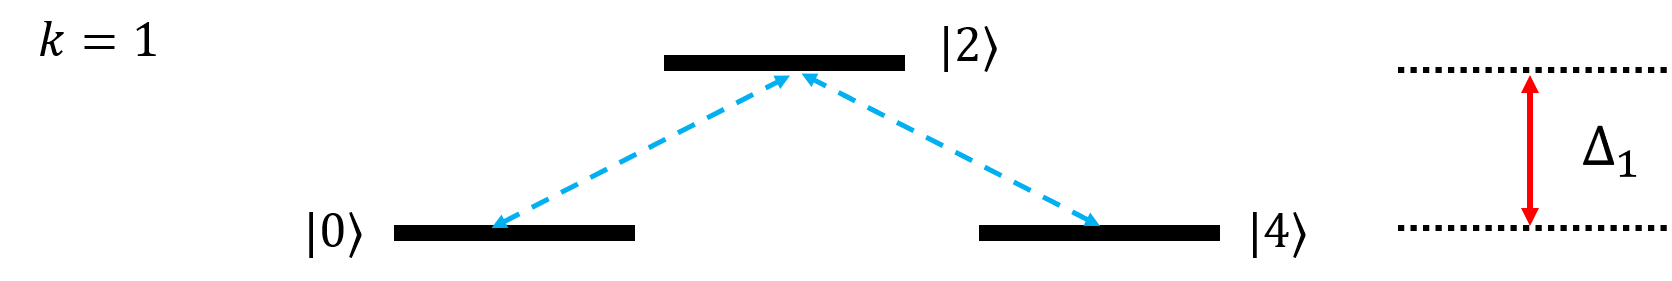
\includegraphics[width=10cm]{file/fig/effective_model/kpo_effective_model_0_4.png}\\
\caption{基底状態と$4$励起状態が縮退する場合のKPOの有効モデル}
\label{fig:kpo_effective_model_0_4}
\end{figure}

$n=8, (k=2)$,すなわち,$0$と$8$が縮退する場合,有効モデルは,図\ref{fig:kpo_effective_model_0_8}のようになり,Hamiltonianの行列表示は,
\begin{align}
     \hat{H}_{\rm{KPO}}^{\rm{eff}}&=
   \bordermatrix{     
    & \bra{0} &  \bra{2} &  \bra{4}&  \bra{6}&  \bra{8} &\bra{10} &\bra{12}\cr
   \ket{0}&E_0&p_1&0&0&0&0&0\cr
  \ket{2}&p_1&E_2&p_2&0&0&0&0\cr
  \ket{4}&0&p_2&E_4&p_3&0&0&0\cr
  \ket{6}&0&0&p_3&E_6&p_4&0&0\cr
  \ket{8}&0&0&0&p_4&E_8&p_5&0\cr
  \ket{10}&0&0&0&0&p_5&E_{10}&p_6\cr
  \ket{12}&0&0&0&0&0&p_6&E_{12}\cr
            }
    %%%
    =
   \bordermatrix{     
    & \bra{0} &  \bra{2} &  \bra{4}&  \bra{6}&  \bra{8} &\bra{10} &\bra{12}\cr
   \ket{0}&0&p_1&0&0&0&0&0\cr
  \ket{2}&p_1&\Delta_1&p_2&0&0&0&0\cr
  \ket{4}&0&p_2&\Delta_2&p_3&0&0&0\cr
  \ket{6}&0&0&p_3&\Delta_1&p_4&0&0\cr
  \ket{8}&0&0&0&p_4&0&p_5&0\cr
  \ket{10}&0&0&0&0&p_5&-\Delta_3&p_6\cr
  \ket{12}&0&0&0&0&0&p_6&-\Delta_4\cr
            }\nn[10pt]
\end{align}
となる.このとき,$E_0=E_8=0$, $p_1=\sqrt{2\cdot1}p$, $p_2=\sqrt{4\cdot3}p$, $p_3=\sqrt{6\cdot5}p$, $p_4=\sqrt{8\cdot7}p$, $p_5=\sqrt{10\cdot9}p$, $p_6=\sqrt{12\cdot11}p$である.である.
\begin{figure}[h]
\centering
		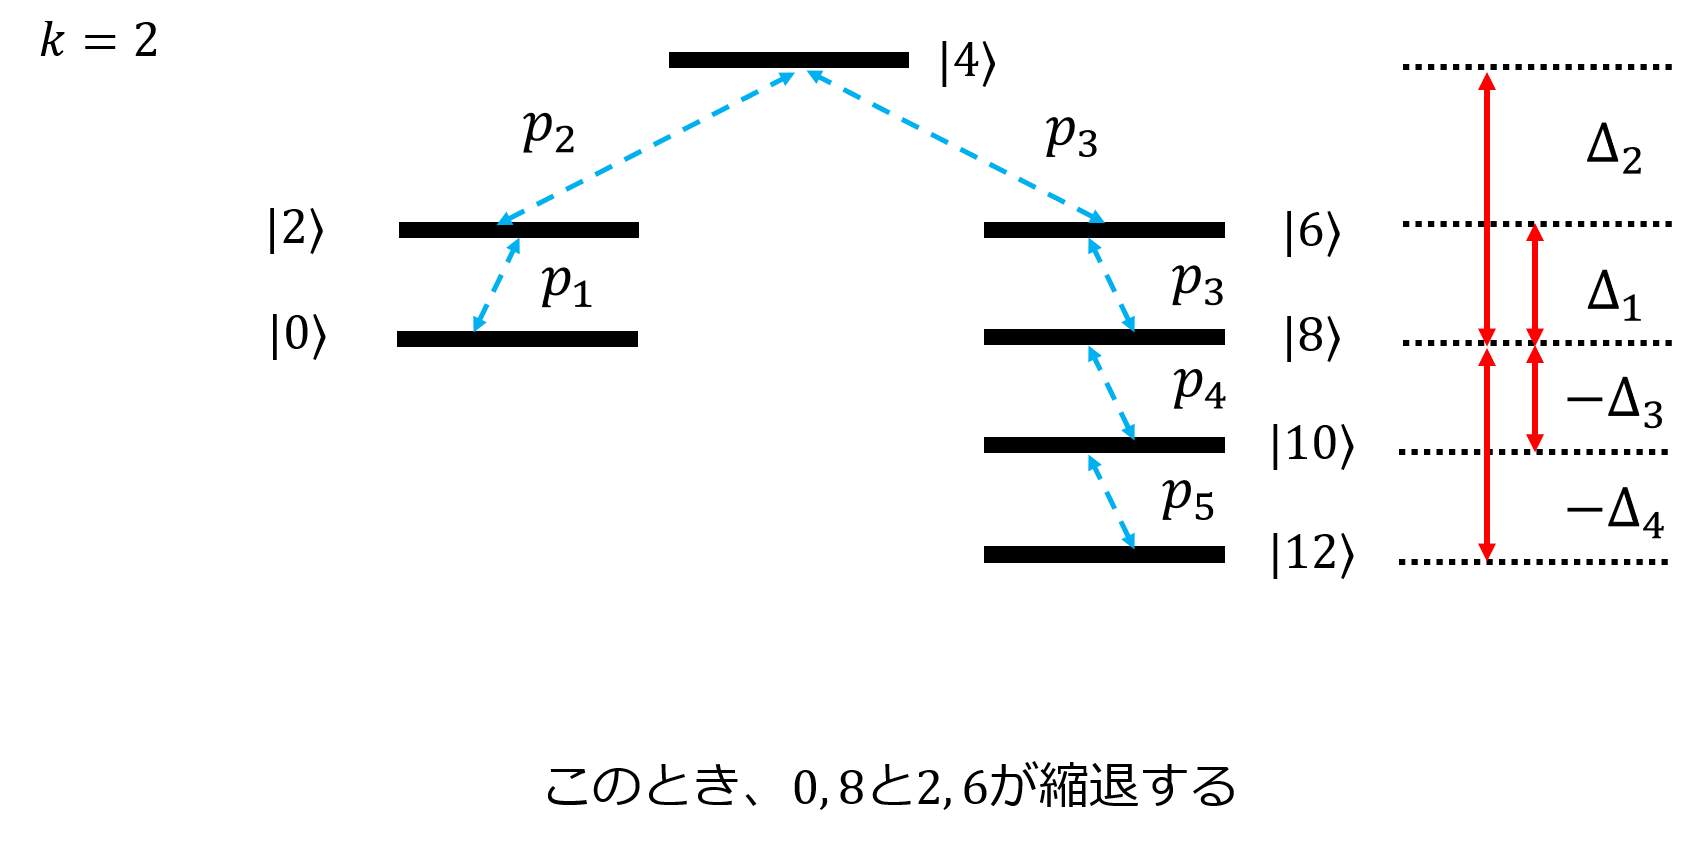
\includegraphics[width=10cm]{file/fig/effective_model/kpo_effective_model_0_8.png}\\
\caption{基底状態と$8$励起状態が縮退する場合のKPOの有効モデル}
\label{fig:kpo_effective_model_0_8}
\end{figure}